\documentclass[12pt]{article}
\usepackage{amsmath,float,booktabs,rotating,graphicx,csquotes}
\usepackage[a4paper,top=2cm,bottom=2cm,left=3cm,right=3cm,marginparwidth=1.75cm]{geometry}
\usepackage[english]{babel}
\usepackage[onehalfspacing]{setspace} % Sets line spacing to 1.5
\usepackage[colorlinks=true, allcolors=blue]{hyperref}
\usepackage[ruled] {algorithm2e}
\usepackage[backend=biber,style=ieee,]{biblatex}
  \addbibresource{references.bib}
\graphicspath{ {./images/} }  % Look within the "images" folder for Images. 

\newcommand{\latex}{\LaTeX\ }
\renewcommand*{\bibfont}{\footnotesize}
\renewcommand*\familydefault{\sfdefault}

\begin{document}
\begin{titlepage}
    \begin{center}
        \vspace*{1cm}
        
\includegraphics[width=0.6\textwidth]{ljmulogo.jpg}
        
        \vspace{0.8cm}
        \huge
        \textbf{Module Title and Module Code}
        \vspace{0.5cm}
        
        \Large
        Title of the Report Topic Area
        
        \vspace{7.5cm}
        
        \large
        A report presented as part of the requirements for\\the BSc (Hons) in Computing\\
        
        \vspace{1.0cm}
        
        School of Computer Science \& Mathematics\\
        Liverpool John Moores University, Liverpool, UK\\
        \vspace{2.0cm}
        Module Leader: Dr. Daniel C. Doolan\\
        
        \vfill
        \today
    \end{center}
\end{titlepage} % Edit the file titlepage.tex to update the Title Page
\clearpage
\singlespacing
\tableofcontents  % Display Table of Contents
\listoffigures    % Display List of Figures
\listoftables     % Display List of Tables
\listofalgorithms % Display List of Algorithms NOTE: may need comment out this line if No Algorithms exist
\clearpage
\onehalfspacing
% The main body / content of the report begins here.

\section{Introduction}
Text text text 

\section{Background Research \& Literature Review}
Text text text

\section{Design}
Text text text

\section{Implementation}
Text text text

\section{Testing and Evaluation}
Text text text

\section{Conclusion}
Text text text

\clearpage % clearpage places the content underneath on to a new page

\section{A Short Guide to Writing and Using \LaTeX} \label{sec:UsingLaTeXGuide}
Should begin with a paragraph introducing the section. 

\subsection{Adding Figures (Images / Graphics) to the Report}

Add an image to the ``\textbf{images}'' folder. Replicate the code in this subsection, which generates Figure \ref{fig:samplepngImage}. Modify the \textbf{label}, \textbf{caption}, \textbf{image file name}, and \textbf{width} to suit. Use the .png format over .jpg for screenshots to avoid image artefacts. 

\begin{figure}[H]
\begin{center}
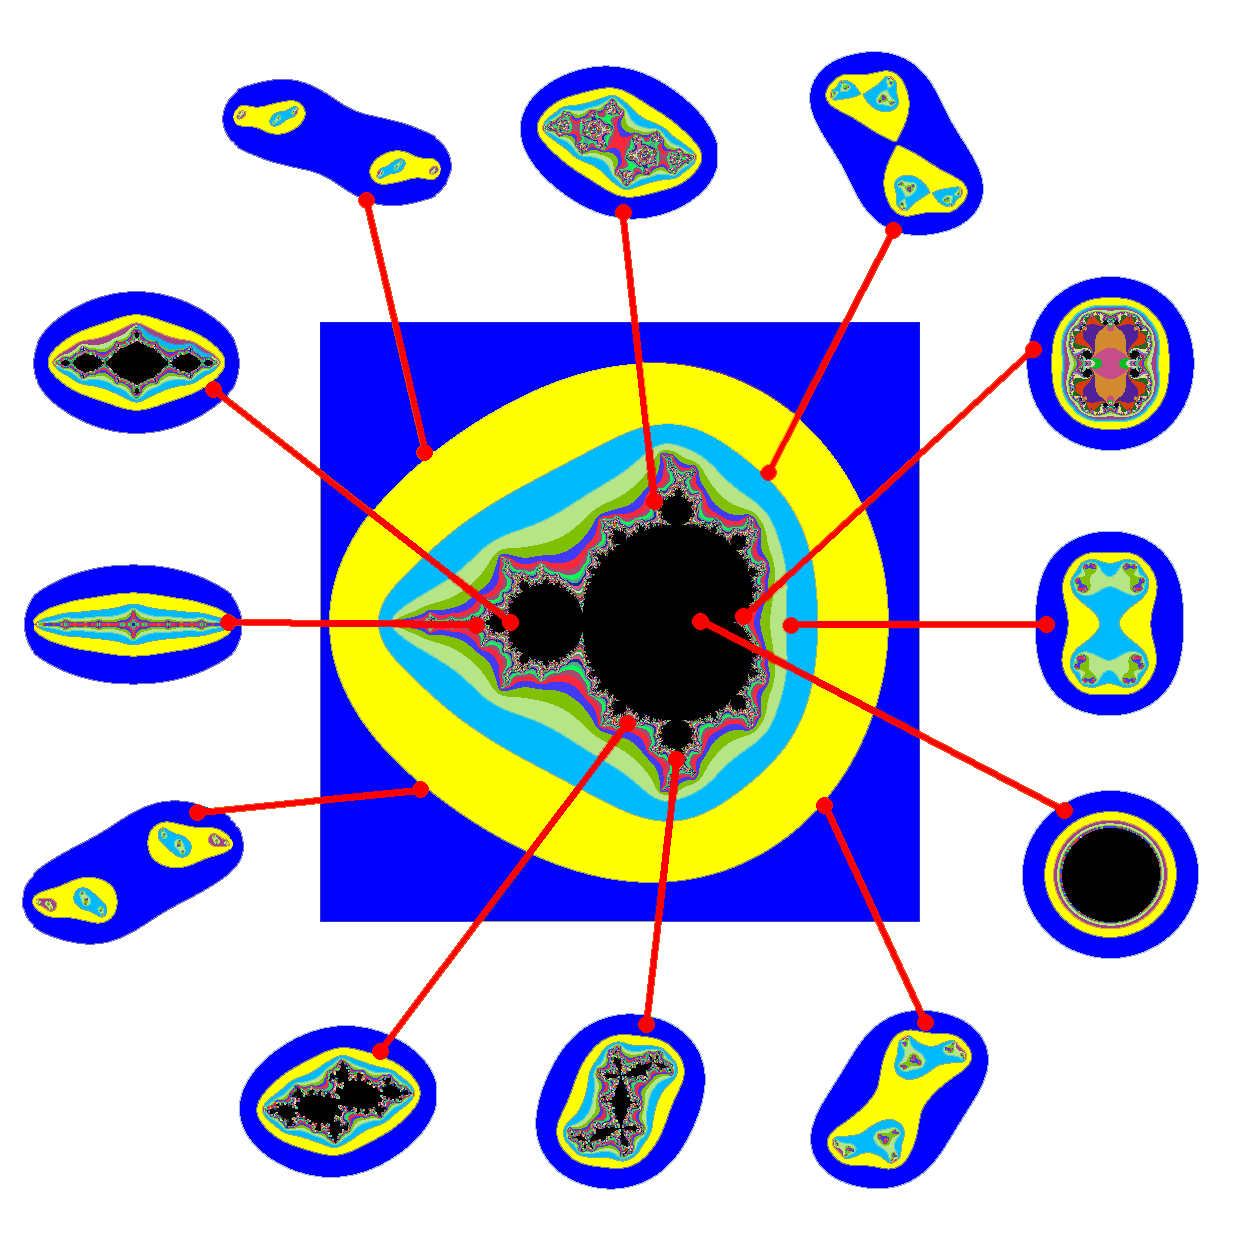
\includegraphics[width=.40\linewidth]{samplepng.png}
\caption{Caption for Bitmap Image (MSet Fractal and Associated JSets)} \label{fig:samplepngImage}
\end{center}
\end{figure}

Figure \ref{fig:VectorGraphicElementPDF} is a Vector Graphic (pdf) file / image. Replicate and edit as needed. Export diagrams in this form to ensure best quality. 

\begin{figure}[H]
\centering
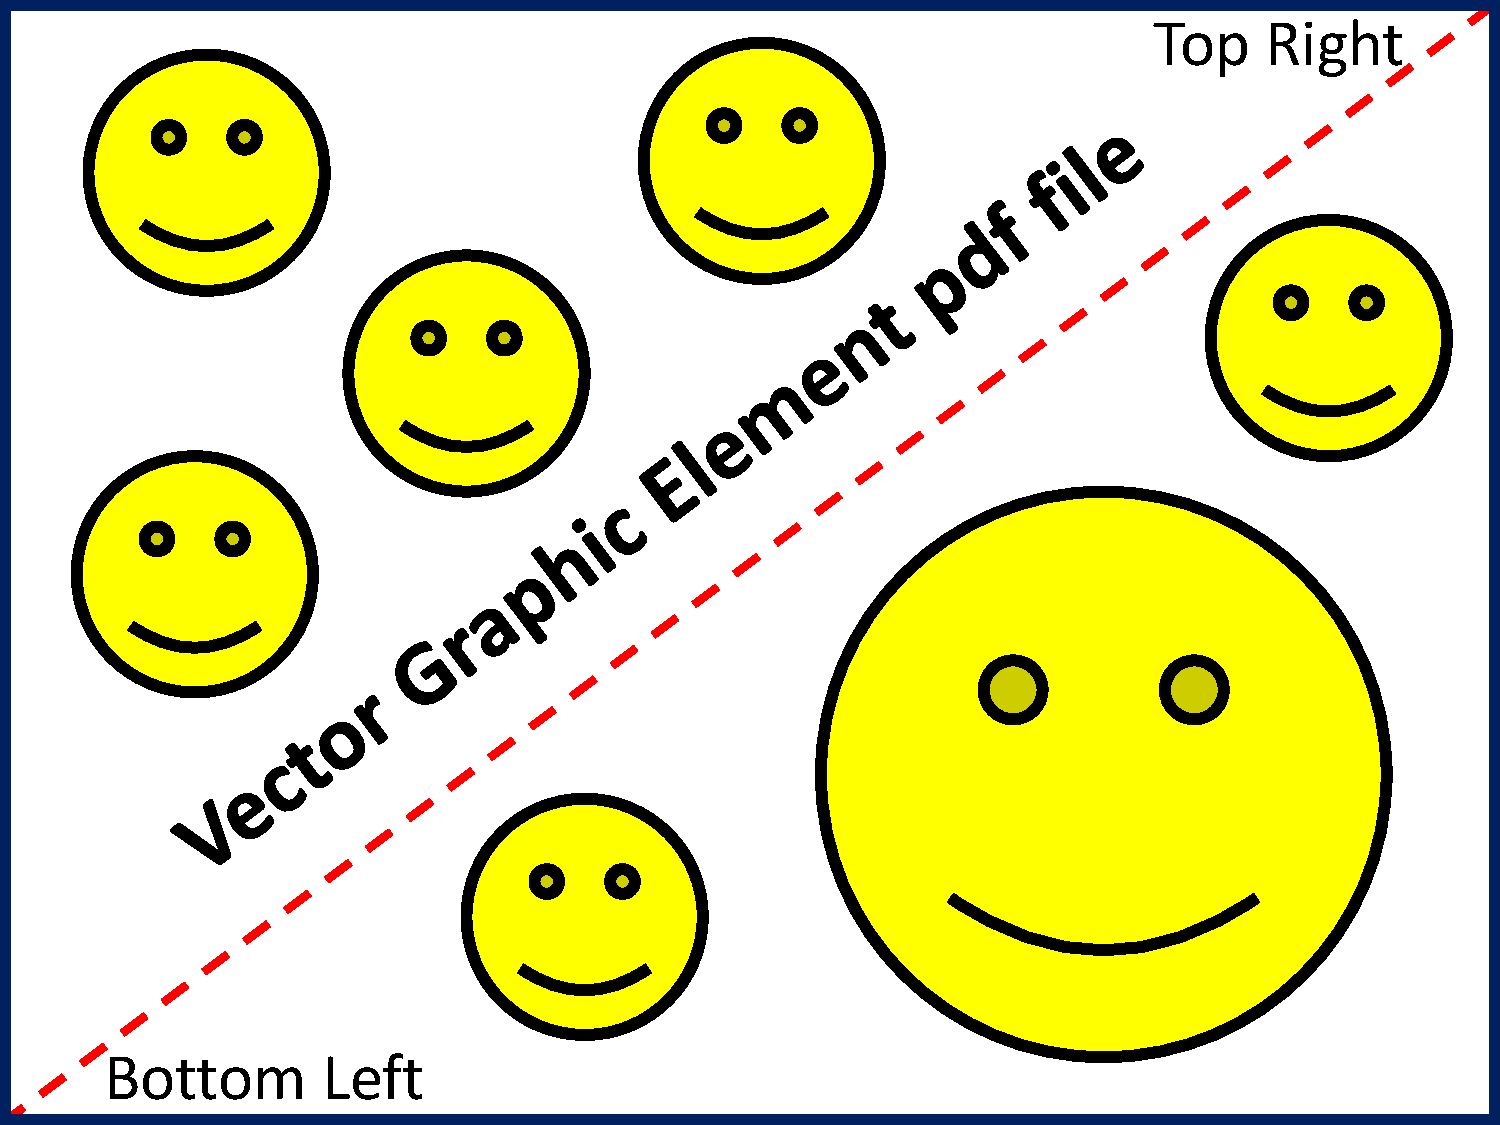
\includegraphics[width=.4\linewidth]{VectorGraphicElementPDF.pdf}
\caption{Vector Graphic - pdf of a PowerPoint Slide}
\label{fig:VectorGraphicElementPDF}
\end{figure}

One may use the \emph{minipage} command when inserting two figures to span across the page. This allows for the subdividing of the page into a number of columns of specified width. Figure~\ref{fig:Example1} \&~\ref{fig:Example2} demonstrate how one may zoom in / focus on a particular section of a graphic by altering the coordinates of the \emph{viewport}. Co-ordinate pairs represent Bottom Left and Top Right of the \emph{viewport}. Replicate and edit as needed. 

\begin{figure}[H]
\begin{minipage}[t]{7.4cm}
\begin{center}
\includegraphics*[viewport= 20 20 600 440, width=.8\linewidth]{VectorGraphicElementPDF.pdf}
\caption{Viewport = 20 20 600 440}
\label{fig:Example1}
\end{center}
\end{minipage}
\hfill
\begin{minipage}[t]{7.4cm}
\begin{center}
\includegraphics*[viewport= 220 200 400 330, width=.8\linewidth]{VectorGraphicElementPDF.pdf}
\caption{Viewport = 220 200 400 330}
\label{fig:Example2}
\end{center}
\end{minipage}
\end{figure}


\subsection{Adding a Table}
Replicate and edit the code as needed, as in the case of  Table~\ref{tab:TableExample}. One should modify the \textbf{label}, \textbf{caption} and \textbf{content} of the table to suit. Cell contents can be aligned to the left (l), right (r), center (c) or paragraph (p). 
\begin{table}[H]
\caption{Place a Caption for the Table Here}\label{tab:TableExample}
\centering
\small
\begin{tabular}{lllp{5cm}}
\toprule \textbf{Heading 1}& \textbf{Heading 2}&\textbf{Heading 3}&\textbf{Heading 4}\\
\midrule
Cell A1 & Cell B2 & Cell C3 & Cell D4\\
Cell E1 & Cell F2 & Cell G3 & Justified text with a defined column size of 5cm\\
\bottomrule
\end{tabular}
\end{table}

\subsection{Citing References to other Articles / Publications}
In this report references are stored in a database with the file name ``{\tt references.bib}''. Replicate and add entries as required, ensuring all have a unique identifier. To cite a reference within the  body text use the \emph{\textbackslash cite} command as per the following examples. Donald Knuth \cite{book:knuth_1973} for example is well known for his work on the Art of Computer Programming. The SETI@Home project \cite{online:berkeleyBOINC} is an example of a webpage citation. One can also work with articles \cite{art:Russell:1978:Cray1}, MSc Thesis \cite{msc:Shannon:1940}, PhD Thesis \cite{phd:Sutherland:1963} or articles within conference proceedings \cite{proc:Ewald:1978:HPG}. Dr. Doolan \cite{online:Doolan:2016:AcademicResources} has provided an online list of resources that may be useful for undertaking literature reviews along with a number of useful \latex tools. 

\subsubsection{References within a Reference Highlighting Pages or other Elements}
To refer to a particular page, section, chapter, equation or other element of a large document add the corresponding information within square brackets right after the \emph{\textbackslash cite} command, such as \emph{\textbackslash cite[p. 2]$\{$online:IEEE-ReferenceGuide:2018$\}$}. Further information is available from the ``IEEE Reference Guide'' \cite[p.3]{online:IEEE-ReferenceGuide:2018}, located in section I.B \cite[Sec I.B]{online:IEEE-ReferenceGuide:2018}. Table~\ref{tab:ReferenceExamples} illustrates a number of common elements one may refer to within a citation, in this case pages or elements of reference ``42'' \cite[Ch. 27]{book:Adams:1979}. It is always useful to check the University Referencing Style Guide for your institution. The IEEE Referencing Style in this template is regularly used in the field of Computing.   

\begin{table}[H]
\caption{Examples of References within a Reference}\label{tab:ReferenceExamples}
\centering
\small
\begin{tabular}{ll}
\toprule \textbf{Reference Type}& \textbf{Presentation Format}\\
\midrule
A Single Page & [42, p. 8] \\
Range of Pages & [42, pp. 4-8] \\
Figure & [42, Fig. 8] \\
Table & [42, Tab. 4] \\
Appendix & [42, Appendix. F] \\
Specific Section & [42, Sec. 4.8] \\
Chapter and Pages & [42, Ch. 4 pp 42-64] \\
An Algorithm & [42, Alg. 4] \\
An Equation & [42, eq. (4)] \\
\bottomrule
\end{tabular}
\end{table}


 

\subsubsection{Referencing Another Element of the Report}
To refer to another part of the document one must use a combination of the \emph{\textbackslash ref} and \emph{\textbackslash label} commands. Section~\ref{sec:WorkWithMath} refers to ``Working with Mathematics'' identified with \emph{\textbackslash label$\{$sec:WorkWithMath$\}$} right after the section heading and referred to here via the instruction \emph{Section$\sim$\textbackslash ref$\{$sec:WorkWithMath$\}$}. 

\subsection{Creating Numeric and Bulleted Lists}
Replicate and edit the code in this subsection to create numbered or bulleted lists. 

{\setstretch{0.85}% Reduces line spacing to compact the list items
\begin{enumerate}
\item First element of a numbered list
\item Second element of a numbered list
\end{enumerate}
\begin{itemize}
\item First element of a bulleted list
\item Second element of a bulleted list
    \begin{itemize}
    \item First nested element of a bulleted list
    \item Second nested element of a bulleted list
    \end{itemize}
\end{itemize}
} % Closing Parenthesis  with respect to the use of \singlespacing for the display of the list elements

\subsection{Working with Mathematics}\label{sec:WorkWithMath}
In line example of the MSet defined as: $Z_{n+1} =
Z_{n}^2 + C$. Matrix Multiplication is typically regarded as an $O(n^3)$
operation, defined in the equation below. One may use the \emph{equation} environment for more complex mathematical formula that should standout. 

\begin{equation}
(A \times B)_{ij} = \sum_{k=0} ^{m-1} a_{ik}b_{kj},~
i=0,...,n-1,~j=0,...,p-1.
\end{equation}

\clearpage

\subsection{Using the Correct Quotes}
To surround a piece of text with double quotes one must place two single quotes on either side of the text. The double quote on the left is created using two left quotes (\lq) this is located just above the \emph{tab} key on the keyboard. The right hand double quote is created using two right hand quotes via (\rq) located just above and to the left of the right shift key. A properly formatted quotation should look like ``This is a quotation''. Notice how the direction of the quotes are opposite to one another. This can be clearly seen in the larger example below. 
\begin{center}
\Huge{``This is a quotation''}
\end{center}
When including text from another source be it online, a book, another report, thesis or other, then it should be surrounded with quotes and a reference to the source provided. 

\subsection{Inserting an Algorithm}
The \emph{algorithm2e} environment \cite{online:Fiorio2016algorithm2e} helps to generate algorithms (Algorithm~\ref{alg:SampleAlgorithm}). If no algorithms are used, then comment out \emph{\textbackslash listofalgorithms } in the file ``{\tt main.tex}'' to remove the list of algorithms heading. Replicate and edit the example code as needed.

\begin{algorithm}
%\dontprintsemicolon
\While{(RANK $<$ COMPSIZE)}{
    \If{(RANK == MASTER)}{
        generate random value \;
        \For{(each item K)}{
            get result \;
        }
    }
}
\caption{A Sample Algorithm in the Domain of Parallel Computing} \label{alg:SampleAlgorithm}
\end{algorithm}

\subsection{What is a Paragraph}
All too often one sees paragraphs comprising of a single sentence, comprising a line or two. Such is inherently not a paragraph. A paragraph should ideally comprise around half a dozen plus sentences, focused on are particular topic of discussion. Often the starting sentence of the paragraph introduces the concept, while the last sentence concludes the discussion put forth. Hence a paragraph should be a cohesive unit of narrative unto itself. This paragraph, not withstanding this sentence, started out by outlining a common problem with paragraphs, then explained the expected structure and concluded that it should be a standalone unit of prose. 

\subsection{Widows and Orphans Anomalies to Avoid when Writing}
These anomalies can occur at the paragraph and page level. A paragraph where a single word or two flows over on to a new line is inherently wasting valuable space on the page. It is thereby worthwhile to review and rephrase the paragraph to avoid such instances \textcolor{red}{occurring.}  

The paragraph above is a good example of such wasted space, take note of the last word of the paragraph ``occouring'', in essence it is positioned all alone, away from all the other words compromising the unit paragraph. 

Another example is where the starting line of a paragraph begins at the end of a page, with the bulk of the paragraph existing on the next page. Making use of \emph{\textbackslash clearpage} can often help, to push the entire paragraph on to the next page. Likewise the last sentence of a paragraph may run over onto the next page. One should again review and rephrase the paragraph as necessary to avoid this, therein maintaining the structural integrity and cohesiveness of the paragraph as a single clearly defined unit. 



\section{Coursework Assignments a Marathon not a Sprint}
Upon release of a coursework start immediately by firstly fully understanding what is required. Make full use of the time provided, making headway straight away, this will provide positive reinforcement and help propel the work along. A good analogy is that of the ``Gym'' or "DevGym" / ``Development Gym of Learning and Skills'' only by the investment of regular and consistent work, will results be achieved. As Gandalf eloquently puts it ``All we have to decide is what to do with the time that is given us'' \cite{book:Tolkien:1991:FOTR}\cite{online:Jackson:2001:FOTR}. 

Professor Randy Pausch is well known for this work on ``Alice 3D'' and his lectures on ``Time Management'' and ``Fulfilling your Childhood Dreams''. Both of these lectures are well worth watching, Dr. Doolan \cite{online:Doolan:2015:PauschLecture} outlines the main elements of both lectures. Dr. Doolan \cite{online:Doolan:2016:SchwarzeneggerInterview} highlights the key elements of success in the form of Goals, Confidence and Time Management. The post once again summarizes and provides links to the key elements of a video interview with Arnold Schwarzenegger. 

\section{Appendix: Rotated Graphics and Tables}
This additional section, in essence an appendix makes use of the \emph{rotating} package to rotate both figures (Figure~\ref{fig:sidewaysFigure}) and tables (Table~\ref{tab:sidewaysTable}) ninety degrees allowing for large data-sets and illustrations to be clearly presented. The images / figures in this template have been provided courtesy of Dr. Doolan (\url{https://dcdoolan.wordpress.com}). Replicate and edit the code of these as needed. 

\begin{sidewaystable}
\begin{center}
   \begin{tabular}{lllllllll} 
   \toprule
   \textbf{Heading 1} & \textbf{Heading 2}  & \textbf{Heading 3}  & \textbf{Heading 4}  & \textbf{Heading 5}  & \textbf{Heading 6}  & \textbf{Heading 7}  & \textbf{Heading 8}  & \textbf{Heading 9}  \cr
   \midrule
   AAAA & BBBB & CCCC & DDDD & EEEE & FFFF & XXXX & YYYY & ZZZZ \cr 
   AAAA & BBBB & CCCC & DDDD & EEEE & FFFF & XXXX & YYYY & ZZZZ \cr 
   AAAA & BBBB & CCCC & DDDD & EEEE & FFFF & XXXX & YYYY & ZZZZ \cr 
   AAAA & BBBB & CCCC & DDDD & EEEE & FFFF & XXXX & YYYY & ZZZZ \cr 
   AAAA & BBBB & CCCC & DDDD & EEEE & FFFF & XXXX & YYYY & ZZZZ \cr 
   AAAA & BBBB & CCCC & DDDD & EEEE & FFFF & XXXX & YYYY & ZZZZ \cr 
   \bottomrule
   \end{tabular}
\caption[A Short Caption for the Table]{
	A much longer caption that will not be listed in the list of tables page.
}
\label{tab:sidewaysTable}
\end{center}
\end{sidewaystable}

\begin{sidewaysfigure}
\centerline{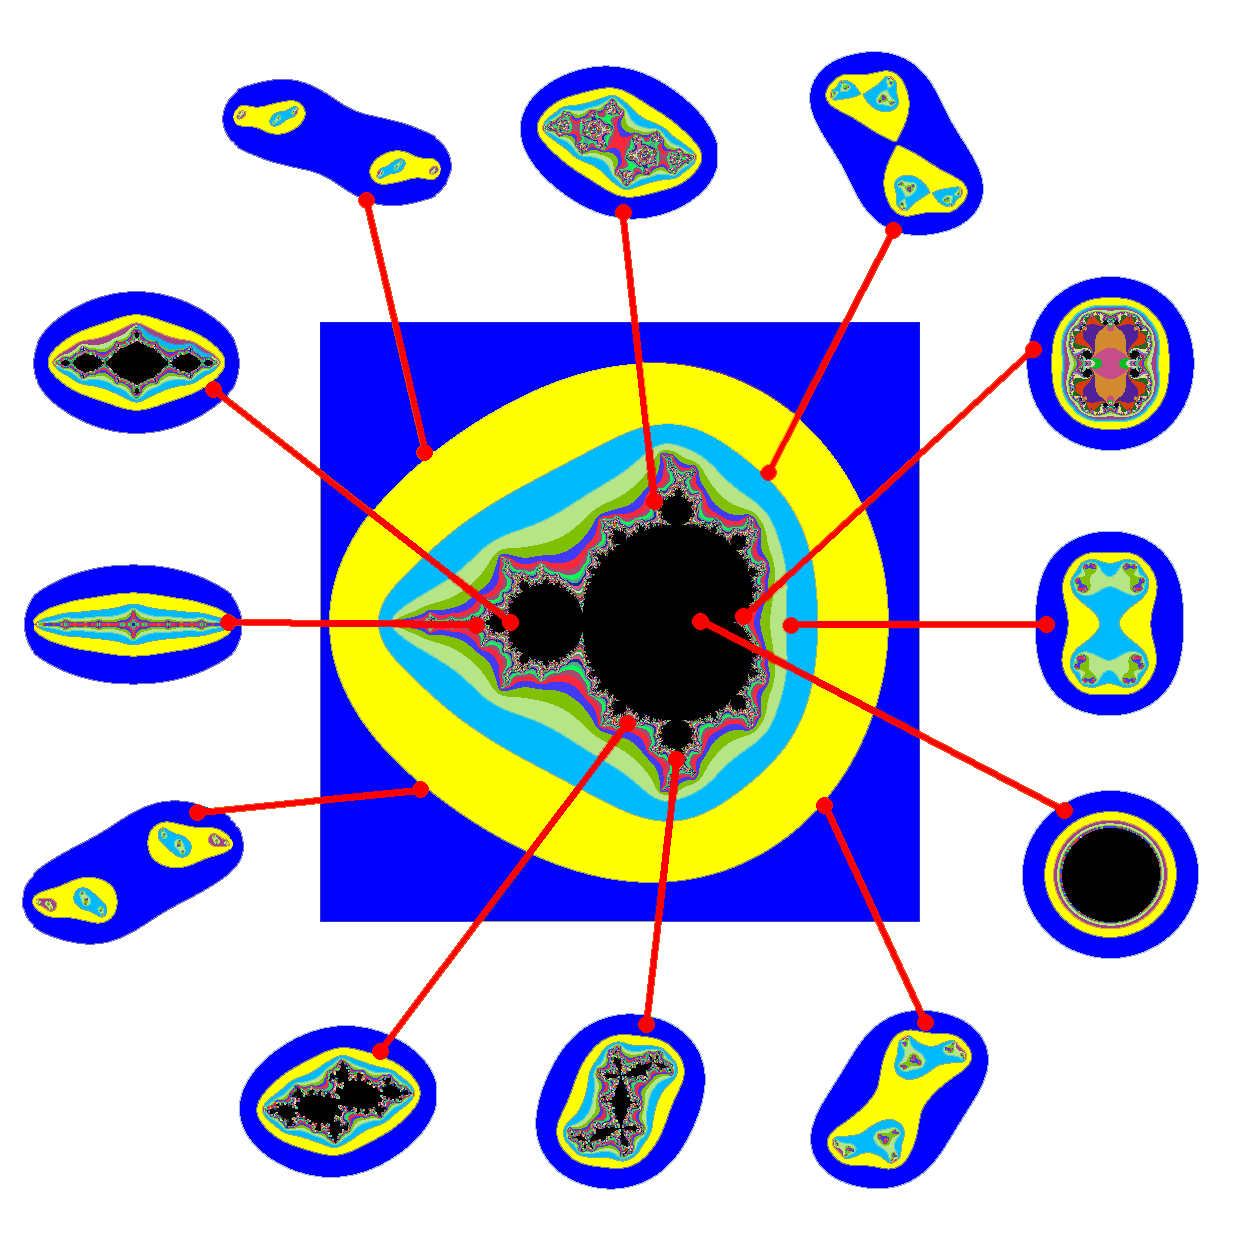
\includegraphics[width=7in]{samplepng.png}}
\caption[A Large Sideways Figure]{
	A much longer caption that will not be listed in the list of figures page (MSet Fractal and Associated JSets).
}
\label{fig:sidewaysFigure}
\end{sidewaysfigure}

 % Add a Percentage Symbol at the start of this line to remove the "How To Guide" from out Compiled pdf

\clearpage
\addcontentsline{toc}{section}{References}
\singlespacing % Reduce the line spacing for the bibliography to save of vertical space usage
\printbibliography
\end{document}